\Chapter{La fusion par confinement magnétique}
\label{AnnexeA}
\begin{refsection}

\section*{La fusion, les tokamaks et le transport transverse}

La fusion thermonucléaire, qui a naturellement lieu dans le coeur des étoiles,
est un processus où deux noyaux atomiques s'assemblent pour former un noyau
plus lourd en dégageant une énergie proportionnelle à la perte de masse suivant
l'équation d'Einstein $E=mc^2$. C'est la source d'énergie la plus prometteuse
à ce jour pour soutenir le besoin croissant en énergie de notre civilisation,
économiquement pérenne, techniquement faisable et écologiquement durable.
Au vu de l'énergie libérée et des sections efficaces de réactions envisageables
entre noyaux, la réaction la plus propice à la production d'énergie est la
fusion deutérieum-tritium (D--T), deux isotopes de l'hydrogène, qui produit une
particule $\alpha$ (une particule d'hélium) et un neutron :
\begin{figure}[!htbp]
    \centering
	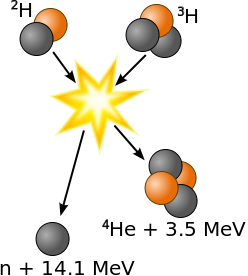
\includegraphics[height=0.5\textwidth]{figures/1-fusion.png}
	\caption{Réaction
de fusion entre le deutérium et tritium suivant l'équation
bilan : $\ce{^2\text{H}}+\ce{^3\text{H}} \rightarrow
\ce{^4\text{H}}\;(3.5\,\text{MeV})+\text{n}\;(14\,\text{MeV})$}\label{fusionDT}
\end{figure}

Cette réaction ne peut se produire que si l'énergie cinétique des particules
dépasse la répulsion mutuelle des noyaux de charge positive (i.e. à des
température de l'ordre de 10 keV à 100 keV, soit plusieurs centaines de
millions de degrés Celcius). L'agitation thermique ayant de plus tendance à
disperser le plasma, celui-ci doit être confiné (i.e. maintenu dans un volume
fini) par des forces extérieures pour atteindre un équilibre favorable à la
réalisation de réactions de fusion.

Afin que la fusion puisse être énergétiquement rentable, il est nécessaire
que l’énergie produite soit supérieure à la somme de l’énergie perdue hors du
système et de celle consommée par les réactions. Cette contrainte, connue sous
le nom de critère de Lawson~\parencite{Lawson}, s'exprime sous la forme
$nT_i\tau_E>f(Q)$ où $n$ est la densité du plasma, $T_i$ la température ionique
et $\tau_E$ un temps caractéristique de relaxation de l'énergie en l'absence de
toute source de chauffage qui mesure la qualité de confinement du plasma. Le
facteur d'amplification $Q$ représente le ratio entre la puissance dégagée par
les réactions de fusion et celle injectée dans le plasma. L'obtention d'un
facteur d'amplification $Q\geq$40 implique par exemple $nT_i\tau_E\geq$~2.7
10$^{21}$~m$^{-3}$.keV.s$^{-1}$.

Deux voies de recherche sont actuellement explorées
pour reproduire la fusion de manière contrôlée :

\begin{itemize}
	\item La fusion par confinement inertiel chauffe compresse des petites
	billes de D--T par des faisceaux lasers intenses pour obtenir un plasma
	extrêmement dense ($n\sim$10$^{31}$~m$^{-3}$) avec un temps de confinement
	d'énergie très court ($\tau_E\sim$10$^{-11}$~s). Les plus grandes
	expérimentations sont le National Ignition Facility (NIF) aux États-Unis et le
	Laser Mégajoule en France.
	\item La fusion par confinement magnétique est au contraire dans l'optique de
	confiner un plasma de densité plus modeste ($n\sim$10$^{20}$~m$^{-3}$) sur des
	temps bien plus longs ($\tau_E\sim$1~s), à l'aide d'un champ magnétique
	intense. Le projet ITER (International Thermonuclear
	Experimental Reactor~\parencite{ITER}), qui est un projet de coopération
	internationale, a pour objectif de construire le premier prototype de
	réacteur à fusion de type tokamak~\parencite{Wesson}, avec un facteur d'amplification
	$Q\geq$10.
\end{itemize}

Le principe des tokamaks fut inventé au début des années 1950 par les Russes Igor Tamm et
Andreï Sakharov. Les tokamaks sont des machines qui utilisent
un champ magnétique de plusieurs Teslas (13T pour ITER) dont les lignes de
champs s'enroulent hélicoïdalement et se referment sur elles-mêmes de façon à ce que le plasma soit
confiné dans un volume fini (cf. figure~\ref{tokamak}).
\begin{figure}[!htb]
    \centering
	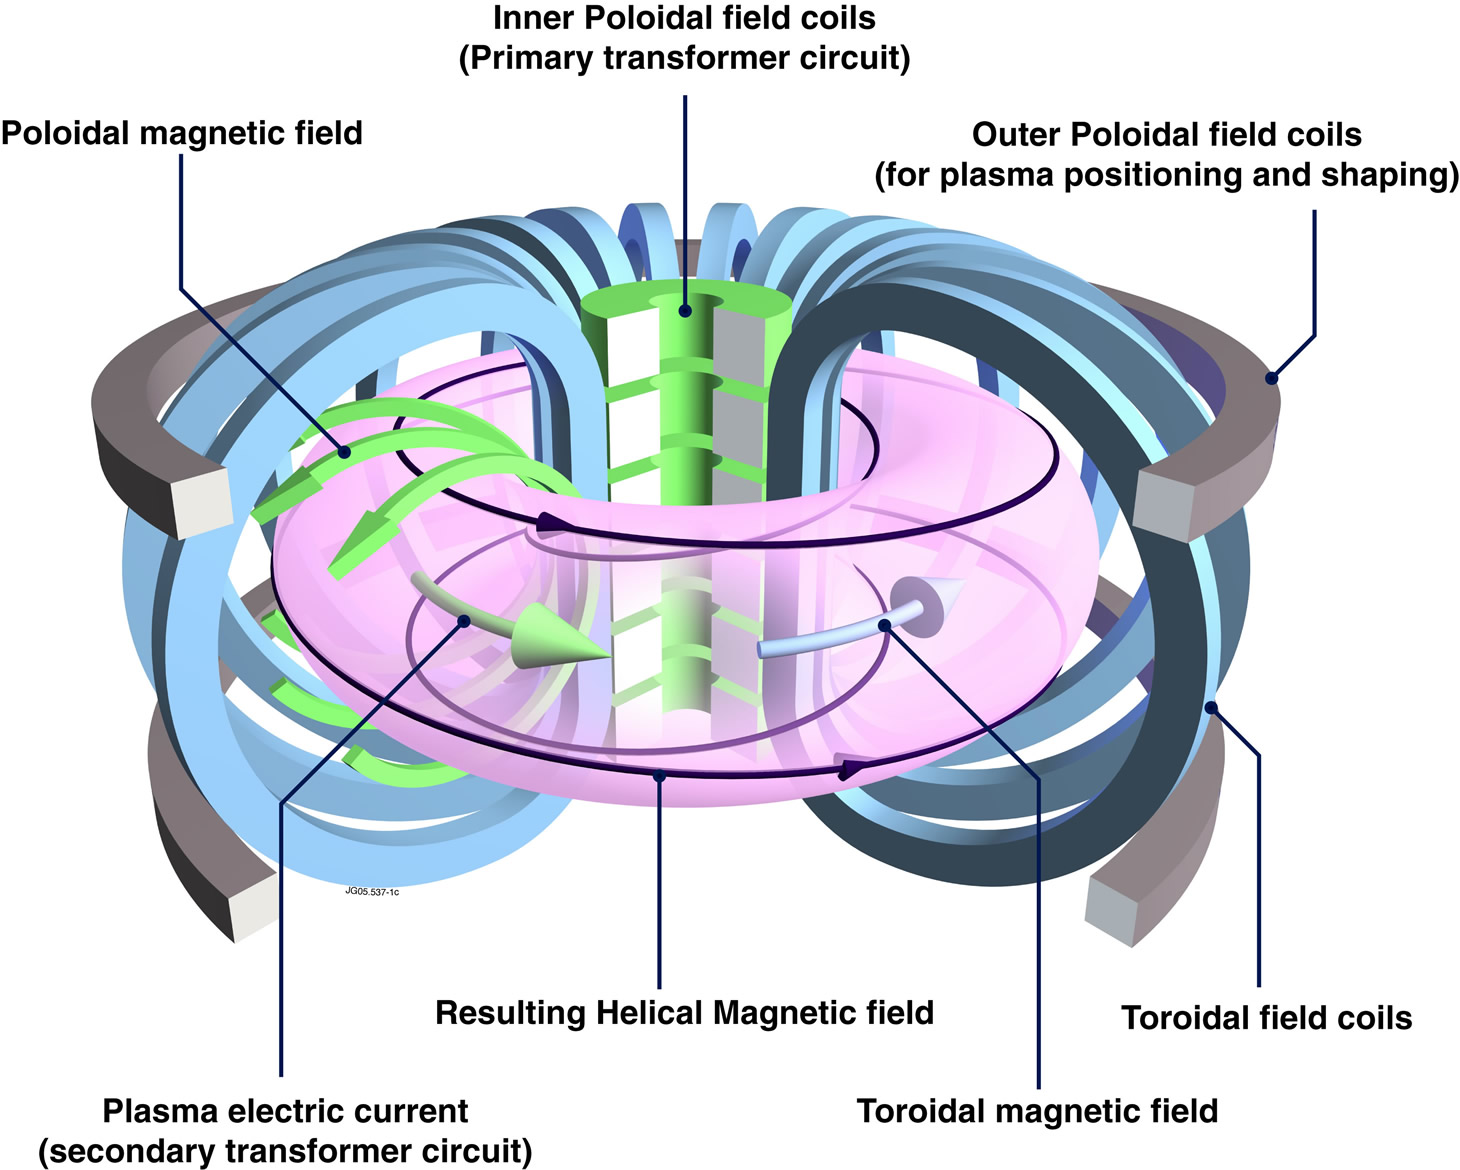
\includegraphics[height=0.75\textwidth]{figures/1-tokamak.jpg}
	\caption{Schéma de principe d'un tokamak. Le terme vient du
russe (toroïdalnaïa kamera s magnitnymi katushkami : en français, chambre toroïdale avec bobines
magnétiques)~\parencite{efda}.}\label{tokamak}
\end{figure}

Le plasma  est créé par chauffage ohmique en induisant un courant
par la décharge du solénoïde central. Le champ magnétique principal, généré
par les bobines toroïdales, confine les particules dans des trajectoires
cyclotroniques autour des lignes de champ. Le courant électrique qui apparaît
dans le plasma, est à son tour à l'origine d'un champ magnétique poloïdal, qui
permet d'obtenir la forme hélicoïdale des lignes de champ (sans laquelle
une lente dérive du plasma dans la direction verticale serait inévitable). Elles
engendrent des surfaces toriques, les surfaces magnétiques.
Enfin, les bobines poloïdales permettent d'ajuster la position et la forme du
plasma.

L'équilibre magnétique, qui résulte du champ magnétique extérieur et du champ
magnétique auto-généré par les courants du plasma, est décrit au moyen des
équations de la MHD (Magnéto-Hydro-Dynamique).
La résolution de ces équations donne accès à la forme et aux propriétés des
surfaces magnétiques. Ce sont des surfaces fermées et emboîtées. Comme le
transport des particules dans la direction parallèle au champ magnétique est de
plusieurs ordres de grandeurs supérieur au transport dans la direction
perpendiculaire, ces surfaces ont la propriété d'être iso-pression,
iso-température, iso-densité et iso-courant.

Le confinement de la configuration tokamak repose sur la rapidité du transport
parallèle par rapport aux processus de transport transverses. Historiquement, le
premier mécanisme envisagé pour décrire le transport transverse est l'existence
de collisions coulombiennes entre particules. Deux particules circulant le long
de lignes de champ voisines peuvent interagir électrostatiquement  et se voir
déviées de leur trajectoire le long d'une autre ligne de champ. L'effet de ces
collisions peut être décrit en terme de diffusion : c'est le transport
classique, de fréquence caractéristique $\nu_{ei}\propto nT^{-3/2}$ et de pas
caractéristique $\rho_{L}$ le rayon de Larmor des particules. Le coefficient de
diffusion classique prend la forme :

\begin{equation}
D_\perp\sim\nu_{ei}\rho_{L}^2
\end{equation}

Selon la théorie classique, c'est le processus dominant de la dégradation du
confinement dans un tokamak. Il suffirait ainsi de réduire $\rho_L$, et donc
d'augmenter le champ magnétique $B$, pour améliorer le confinement.
Malheureusement, les mesures expérimentales montrent que les coefficients de
transport de la chaleur et des électrons sont de plusieurs ordres de grandeurs
supérieurs à ceux prédits par la théorie classique. En ce qui concerne le
transport de matière, les observations rapportent en effet des coefficients de
diffusion de l'ordre de celui de Bohm, défini par :

\begin{equation}
D_\text{Bohm} \equiv \rho_L v_{T} \sim T/qB
\end{equation}

où $v_{T}$ est la vitesse thermique des particules, $T$ leur température, $q$
leur charge et $B$ l'intensité du champ magnétique. Le rapport typique des
valeurs expérimentales et classiques est $D_\perp/D_\text{Bohm}\,$=~10$^{-2}$.
Parce qu'il n'était pas expliqué dans le cadre de la théorie classique, ce
transport a reçu le nom de transport anormal.

Il est aujourd'hui communément admis que ce fort transport transverse est
d'origine turbulente. Avec en point de mire l'amélioration du confinement pour
satisfaire le critère de Lawson, théoriciens et expérimentateurs travaillent
depuis plusieurs années à la compréhension des mécanismes et
caractéristiques de la turbulence.

Signalons enfin qu'un trop bon confinement n'est pas souhaitable : l'énergie
produite dans les réaction de fusion doit bien être récupérée, et il faudra
également veiller à l'extraction des impuretés et des cendres d'hélium.

Pour toutes ces raisons, le contrôle du transport transverse et donc de la
turbulence est un des enjeux majeurs des machines à fusion magnétique. Il passe
par la compréhension de son origine, et la détermination de ses
caractéristiques.
\end{refsection}
